%!TEX program = lualatex
\documentclass[conference, 10pt, a4paper]{IEEEtran}

\usepackage{hyperxmp}

\usepackage{ifluatex}
  \ifluatex
    \usepackage{fontspec}
	\usepackage{polyglossia} % babel replacement for use with fontspec
	\setdefaultlanguage[variant=american]{english}
	\selectlanguage[variant=american]{english}
  \else
    \usepackage[utf8]{inputenc}
    \usepackage[T1]{fontenc}
	\usepackage[american]{babel}
  \fi

\usepackage[acronym, nomain, nowarn]{glossaries}
\loadglsentries{acronyms}
\usepackage{booktabs}
\usepackage[hyphens]{url}
\usepackage[pdfhighlight=/O, hidelinks, unicode=true]{hyperref}
\usepackage{mathtools}
\usepackage{fixmath}
\usepackage{algorithm2e}
\usepackage{subcaption}
\usepackage[load-configurations={abbreviations,binary}, per-mode=symbol]{siunitx}
\sisetup{load-configurations = abbreviations,binary-units}
\usepackage{tabu}
\makeglossaries
\usepackage[url=false,doi=false,backend=biber,style=ieee,sorting=none,minnames=1,maxnames=6]{biblatex}
\addbibresource{literature.bib}
\usepackage[inline]{enumitem}

\hypersetup{
pdftitle = {Understanding Online Video Games in Order to Improve QoS Measurements},
pdfauthor = {Florian Metzger, Tobias Hoßfeld}
}


\makeatletter
\newcommand{\removelatexerror}{\let\@latex@error\@gobble}
\makeatother

\begin{document}

%\title{Things to Keep in Mind When Measuring Online or Streamed Video Games}
%\title{QoS Measurement Approaches for Online Video Games from Basic Game Mechanics}
%\title{Best Practices for QoS Measurements of Online Video Games}
\title{Understanding Online Video Games in Order to Improve QoS Measurements}

\author{\IEEEauthorblockN{Florian Metzger\IEEEauthorrefmark{1}, and Tobias Hoßfeld\IEEEauthorrefmark{1}}
\IEEEauthorblockA{\IEEEauthorrefmark{1}
Chair of Modeling of Adaptive Systems\\
University of Duisburg-Essen\\
Essen, Germany\\
\{florian.metzger,tobias.hossfeld\}@uni-due.de}}

\maketitle

%!TEX root = paper.tex
%%%%%%%%%%%%%%%%%%%%%%%%%%%%%%%%%%%%%%%%%%%%%%%%%%%%%%%%%%%%%%%%%%%%%%%%%%%%%%%%
\begin{abstract}

Recently, online and cloud video games have been shifting into the 
focus of consumer and academic interest. 
%Online and cloud gaming might 
%be the next-big-thing after HTTP adaptive video streaming for the 
%fields of computer network performance evaluation and \acrshort{QoE} 
%modeling it. A quickly growing number of publications concerns itself 
%with assessing the subjective quality of those two game types. 
However, 
due to the nature of video games and their large diversity, assessments 
of subjective game quality  
are always specific to a single game, and arguably even specific to the 
exact experiment conditions, and are difficult to
transfer to any other game, even if they seem to be similar on the 
surface.

This paper aims to rectify this by providing a model for an underlying 
mechanic that is a governing property of most of such earlier results: 
The end-to-end lag of video games. The paper describes in detail the 
components of this lag model, and additionally provides a 
parametrizable simulation that calculates the lag.

Open Access Notice: The authors explicitly encourage the review and 
reuse of all the data and custom tools used in the preparation of 
this paper. The materials are available from the authors' public 
repository \cite{mas-ude-github}. 

% The online interactions and resulting user experience of the online 
%interaction of video games have been a topic of several publications in 
%the past. This trend was reinforced through the development of Cloud 
%Gaming with its strong dependence on good network conditions. Many of 
%these studies focus on subjective user assessments, as this is usually 
%an approach that quickly results in usable scores without going too 
%deep into technical details of video games. Contrary, objective and 
%\acrshort{QoS}-centric measurements are often much harder to conduct.

% This paper aims to offer some insights and best practices for the 
%realization of such objective online video game measurements. To 
%facilitate this, we first discuss two properties intrinsic to video 
%games which distinguish them from pure video streaming:
% \begin{enumerate*} 
% 	\item the framerate and 
% 	\item the game tickrate 
% \end{enumerate*}
% and their impact on the game's interactivity and end-to-end lag. 
%Derived from these properties three distinct measurement approaches and 
%their limitations are presented.

\end{abstract}

%!TEX root = paper.tex
%%%%%%%%%%%%%%%%%%%%%%%%%%%%%%%%%%%%%%%%%%%%%%%%%%%%%%%%%%%%%%%%%%%%%%%%%%%%%%%%
\section{Introduction}
\label{sec:introduction}

Recently, video games have garnered research interest from both the computer networking and the \gls{QoE} communities, focusing on network-related properties and the resulting \acrshort{QoS} and \gls{QoE} of individual video games. 
% Many of these research efforts were triggered through the contrivance of cloud gaming, though the user experience of online games still remains a topic of investigation and research. 
A quickly growing number of publications also concern themselves with assessing the \gls{QoE} of such games. These assessments are usually conducted through user studies, and when set up correctly they can produce meaningful results. However, the inherent diversity of games and their accompanying gameplay mechanics make it difficult to transfer any of these results from one game to another. In contrast to passively consuming videos, games are highly interactive, making the setup of such studies much more difficult. Compared to plain video streaming, underlying properties of video games are also not straight-forward to observe from the outside. Yet, in order to conduct proper measurements, it is essential to understand them. This work aims critically questions from past gaming user studies and derive lessons learned them as well as to give insights into some of gaming's core properties. To further this, an \gls{E2E} lag model is introduced which represents the lag between a user input event and the display of the event's results on the screen. The model describes game lag on the basis of other intrinsic game factors, such as the framerate and tickrate. Initial results with this model confirm the influence of framerate and tickrate on the \gls{E2E} lag and therefore also on the game's subjective interaction quality. This means that these two parameters need to be tightly controlled in subjective quality assessment studies.

%!TEX root = paper.tex
%%%%%%%%%%%%%%%%%%%%%%%%%%%%%%%%%%%%%%%%%%%%%%%%%%%%%%%%%%%%%%%%%%%%%%%%%%%%%%%%
\section{Related Work}
\label{sec:relatedwork}


The assessment of video games has been a topic in many past papers. Due to the strong interactivity of games and the large number of different game mechanics most of the research is focused on conducting user studies and noting the subjective quality of the users. But the outcome of these studies still depends very much on a wide selection of factors, e.g., on the precise setup, the game, and the choice of players, that make comparing their results to each other quite difficult. This section presents a few examples of such studies.

In \cite{5976180} Jarschel et al. identify some influence factors on the subjective quality of cloud gaming through a user survey for certain games and three different game categories (slow, medium, fast games) that have been subjected to worsening \gls{QoS} parameters. Downstream packet loss and delay was noted be be especially problematic for achieving a good quality. Similarly, the authors of \cite{4591393} observed the relationship of players quitting a \gls{MMO} game with deteriorating \gls{QoS} and noted an impact proportion of 1:2:4:3 for delay, jitter, and packet loss on both the client-to-server and server-to-client connections respectively. Additionally, a user study in \cite{4604397} also showed a correlation of the \gls{QoE} to the delay as well as the jitter for another \gls{MMO}, in this case the total delay had more impact than the delay variation. Regarding the subjective quality in first person shooters, the authors of \cite{6614351} find a strong impact of the delay and packet loss on the experienced quality. The authors of \cite{6404025} and \cite{beyerusing} use \gls{fEMG} and \gls{EEG} approaches respectively to examine individual gamers' reaction to various cloud games and measure the quality they are experiencing in terms of real-time strictness and \gls{QoE}. Finally, an ITU-T Recommendation \cite{mollertowards} concerning subjectively measuring video game \gls{QoE} is also in preparation, which discusses game-relevant \gls{QoS}-metrics as well as the selection of players and games.

In order to avoid some of the issues with subjective user studies other approaches examine the players' objective performance through in-game metrics such as the game's highscore or the duration to achieve a certain task. For example, a user study in \cite{Chen:2006:SOG:1167838.1167859} observes a decrease in the objective quality assessment metrics (the playing duration) in an \gls{MMO} due to the influence of network factors. A 2006 paper \cite{Claypool:2006:LPA:1167838.1167860} categorizes player actions and their relationship to latency, with special regards for the actions' precision as well as their deadline. However, the in-game metrics under study can not represent short-term effects of latency as they operate on much larger time-scales. 
%(e.g. researching the whole technology tree in Warcraft 3 is neither a representative action of the game nor delay-sensitive at all). Also the presence of lag compensation techniques is not considered. The end result is a delay tolerance table which probably is not very representative of modern video games.
A second paper by Claypool et al. \cite{claypool2007} furthers this notion of the influence of network \gls{QoS} on in-game actions and specifically looks at players' performance in first person games. A user study records the performance in artificially created in-game environments. Here, the performance gets worse with a degraded network, albeit at a very slow pace. %Players were also subjected to very low framerates of \SI{7}{\hertz} and \SI{3}{\hertz}, which is such an unrealistic setting, that it should not even have been tested. The reasons for this are laid out in Section~\ref{sec:framerate}.
The ``kills per minute'' of normal players in the \gls{FPS} \textsc{Quake 3} are investigated by \cite{1266180}, which sees a steady decline of this subjective performance metric when increasing the network delay. However, another paper \cite{Beigbeder:2004:ELL:1016540.1016556}, looking at player performance in \textsc{Unreal Tournament 2003} in a controlled in-game environment, finds almost no influence of increased delay and packet loss, even at high values of \SI{200}{\milli\second}. %The discrepancy between the otherwise similar studies could potentially be attributed to the specific construction of the in-game test environment. 
A 2002 paper \cite{Pantel:2002:IDR:507670.507674}, which gathered objective \gls{QoE} measurements from a custom-made RC racing video game, again sees a strong dependence of the player's performance on the delay, and suggests that a network \acrshort{RTT} of \SI{200}{\milli\second} is barely usable and \SI{500}{\milli\second} completely unusable. Finally, the authors of \cite{Bredel:2010:MSR:1944796.1944797} also find a strong and negative influence of high delay on the player's performance, in this case again in \textsc{Quake 3}. 

It is interesting to note the discrepancies both in terms of the influencing parameters as well as their degree in between the studies. Considering the complexity and variability of video games and the difficulties of finding and setting up good comparable scenarios and testbeds, it is understandable that some studies come to different results. This makes it much more important to first understand the basic components and underlying objective metrics. Quality estimations of video games could be much more representative if models for these metrics would exist to easily understand their influences without having to conduct a full user study.





%Pure \gls{QoS} views on the quality of online video games are rather are, but are nonetheless important in correctly assessing any game-related parameters and are also the foundation for most objective and subjective \gls{QoE} studies.



%A 2012 article notes the dependence of gaming on latency and the difficulties cloud-based solutions have in providing a sufficiently low latency. The suggest a move closer to the edge to reach more users in a quality they deem adequate.  \cite{Choy:2012:BSC:2501560.2501563}.
%``The Brewing Storm in Cloud Gaming: A Measurement Study on Cloud to End-user Latency'' 

%``Placing Virtual Machines to Optimize Cloud Gaming Experience'' \cite{6853364}  interesting for cloud gaming economics

%Adaptive Mobile Cloud Computing to Enable Rich Mobile Multimedia Applications \cite{6413270}

%Addressing Response Time and Video Quality in Remote Server Based Internet Mobile Gaming \cite{5506572} optimize mobile cloud gaming based on a certain impairment function and by reducing video bitrate and fps (even sub 10fps...)

%``Kahawai: High-Quality Mobile Gaming Using GPU Offload'' \cite{Cuervo:2015:KHM:2742647.2742657}

%``Outatime: Using Speculation to Enable Low-Latency Continuous Interaction for Mobile Cloud Gaming'' \cite{Lee:2015:OUS:2742647.2742656}

%``Assessing the Impact of Game Type, Display Size and Network Delay on Mobile Gaming QoE'' \cite{beyer2014typedisplaydelayimpact} Another user study regarding context factors like screen size and their impact on MOS, but also game type and delay on MOS

%A Method For Feedback Delay Measurement Using a Low-cost Arduino Microcontroller \cite{beyermethod} already covered in measurement methods section

%``QoE Assessment of Interactivity and Fairness in First Person Shooting with Group Synchronization Control'' \cite{Ida:2010:QAI:1944796.1944806} interessant für lag compensation betrachtungen

%``The Impact of Video Encoding Parameters and Game Type on QoE for Cloud Gaming: a Case Study using the Steam Platform'' \cite{slivarimpact}

%``How Do New Visual Immersive Systems Influence Gaming QoE?'' \cite{hupontnew} Vergleich Immersion am monitor vs oculus. beispiel eines schlechten testsetups, da unterschiedliche FoV für beide ausgabetypen (75° vs 100°), test wird stark verfälscht

%%``An experimental estimation of latency sensitivity in multiplayer Quake 3''  vs. \cite{1266180} ``The Effects of Loss and Latency on User Performance in Unreal Tournament 2003'' \cite{Beigbeder:2004:ELL:1016540.1016556}. both papers completely contradict each other: Quake 3: significant impact of latency on game performance (kills/minute); UT3: no impact on user performance at all (kills/deaths per game)

%``Security issues in online games'' \cite{doi:10.1108/02640470210424455}
%!TEX root = paper.tex
%%%%%%%%%%%%%%%%%%%%%%%%%%%%%%%%%%%%%%%%%%%%%%%%%%%%%%%%%%%%%%%%%%%%%%%%%%%%%%%%
\section{Fundamental Game Properties}
\label{sec:gamemechanics}

This section will focus on describing the main game loop and the 
framerate and both their implications for properly measuring video 
games. On a technical level these two properties distinguish passively 
consumed videos and video games the most.


%%%%%%%%%%%%%%%%%%%%%%%%%%%%%%%%%%%%%%%%%%%%%%%%%%%%%%%%%%%%%%%%%%%%%%%%%%%%%%%%
\subsection{The Framerate}
\label{sec:framerate}

In contrast to traditional video media with their fixed framerates of, 
e.g., \SI{24}{\hertz} or \SI{29.97}{\hertz}, video games are more 
flexible but simultaneously also much more demanding to the framerate. 
Generally speaking, motion in video data is based on the principle of 
\textit{apparent motion}. In order to perceive objects to be in motion 
in videos, consecutive images have to appear at a certain rate which is 
considered to be at about \SI{16.67}{\hertz} according to 
\cite{wertheimer1912experimentelle}. Below that threshold objects will 
appear as two distinct objects between two consecutive frames.
%This form of apparent movement is called the phi phenomenon.
The higher the rate of displaying images, the more fluid the motion 
looks, as the discrete ``jumps'' in the position of the object get 
smaller the higher the framerate is.\footnote{One can verify this 
behavior for example at \url{https://frames-per-second.appspot.com/}.}.

In general, there is no commonly established upper limit to the 
framerate that humans can still perceive as an improvement to motion 
presentation, the gain has however diminishing returns. The typical 
movie framerate of \SI{24}{\hertz} is considered to be at the lower end 
of motion perception but mostly still works without any problem due to 
the presence of motion blur. This artifact is always present in 
recorded images as objects are still in motion during film exposure.
%A faster shutter speed reduces the amount of motion blur.
% film grain also has an influence

% \begin{figure}[!t]
% 	\centering
% 	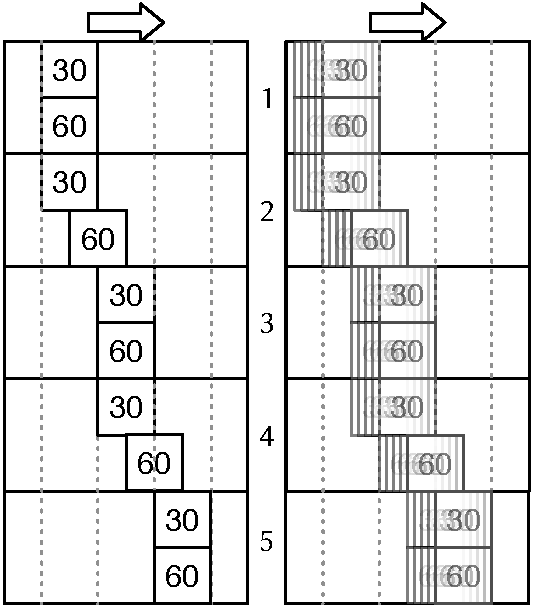
\includegraphics[width=1.0\columnwidth]{images/framerate.pdf}
% 	\caption{Effects of frame rate and motion blur on the smoothness of 
%movement and spatial resolution. Objects move at the same speed to the 
%right only the position os updated at different rates. A depiction of 
%strong motion blur was added to the right-hand side.}
% \label{fig:framerate}
% \end{figure}

The benefit of motion blur lies in its ability to conceal stutters in 
apparent movement due to the object and its edges being blurred, 
thereby reducing the positional information available on it.
%, Figure~\ref{fig:framerate} illustrates this. 
Therefore, typical movie sequences usually appear to be perfectly 
fluid. Only for example when the camera pans at a high speed stutters 
in object movement or the viewport updates become apparent. Intrinsic 
motion blur is absent in computer generated imagery but can be 
artificially added to the images. While adding blur to video games can 
improve fluidity, it also reduces the spatial information available to 
the player and hampers the precision of the player's actions. Therefore 
it is often avoided, especially for objects in focus.

Video games add two more factors to the frame rate consideration. The 
first is the issue of the monitor's refresh rate. Monitors work with a 
fixed, configurable image refresh rate, typically always including 
\SI{60}{\hertz}. If the game outputs images at an inconsistent rate or 
a rate lower than the monitor's refresh rate or if the framerate is not 
an integer multiple of the refresh rate or vice versa one of two things 
will happen:
%(depending on the implementation and the presence of vsync)

\begin{itemize}
	\item If the monitor fetches a frame from the graphics card's buffer 
while the frame is still being rendered, the result will be a mixture 
of the new frame in the upper half of the image and a frame which is 
one time interval older. This artifact is called \textbf{tearing} and 
should be avoided.
	% only the upper portion of the frame  finished, One frame split up 
%between two refresh cycles
	\item Games can also be configured to postpone the rendering of a new 
frame until the monitor has already fetched and displayed the current 
frame, this is called waiting for vertical synchronization or 
\textbf{VSYNC}. No tearing will occur, but the \gls{IAT} of new frames 
might become very irregular, displaying some frames more often than 
others just to match the monitors refresh rate, resulting in a 
stuttering display. This latter stuttering effect also occurs for 
\SI{24}{\hertz} movies being displayed on a \SI{60}{\hertz} TV screen. 
Therefore most TVs additionally provide a dedicated \SI{24}{\hertz} 
refresh rate mode to remove the stuttering.
\end{itemize}

Finally, video games also distinguish themselves from video material by 
being highly interactive. Specifically this means that video games 
constantly require inputs on short time scales to which the game reacts 
and displays the feedback. Therefore, the framerate also influences the 
reactivity of a game and can be a source of latency as discussed 
further in Section~\ref{sec:latency}.


%%%%%%%%%%%%%%%%%%%%%%%%%%%%%%%%%%%%%%%%%%%%%%%%%%%%%%%%%%%%%%%%%%%%%%%%%%%%%%%%
\subsection{Game Tick Rates and Send Rates}

At their core video games are essentially feedback-directed real-time 
simulators. The simulator's main loop consists of three central parts 
as depicted in Fig.~\ref{alg:gameloop1}. Every render-call means 
putting out a new video frame. As this framerate is usually not limited 
and variable, the game logic has to update its state on a time-scale 
operating independent of the current frame. Some games also update 
parts of the game on a fixed frequency, the so-called 
\textbf{tickrate}, for example a non-game-influencing physics effect 
updating at a lower \SI{30}{\hertz} rate.

%Some games do not do this and tie the game time directly to the frame 
%rate and expect to be run at a fixed frequency. If one manages to 
%unlock the frame rate in such games, the game will often run much 
%faster with numerous mostly disadvantageous side effects. Examples 
%include games optimized for older CPUs and clock speeds now 
%unexpectedly running at much higher clocks. Also games such as Need for 
%Speed Rivals, which was locked at 30 fps, but could be unlocked and 
%subsequently behave erroneously. Also, games with a locked frame rate 
%are very much frowned upon in the gaming community, especially when the 
%cap is lower than 60 fps.
%This general logic is also preserved in modern multi-threaded game 
%designs, although it is more difficult to achieve.

\begin{figure}[!t]
\centering
\removelatexerror
\begin{algorithm}[H]
 \While{game running}{
  read inputs\;
  update game state\;
  render screen\;
 }
\end{algorithm}
\caption{Basic model of a continuous main video game loop.}
\label{alg:gameloop1}
\end{figure}

Online video games complicate this update logic a bit. In online games, 
the client is not the final authority over its game state any more. 
Instead, interpreted input commands are sent to the server and a 
preliminary game state is calculated locally. When the authoritative 
update from the server is received the two states can be once again be 
synchronized. A typical scenario with all the relevant rates for an 
online game running in a cloud gaming environment is depicted in 
Fig.~\ref{fig:tickrate-streamed}. To make matters even more complicated 
the rates of sending input commands from the clients to the server as 
well as game state updates from the server to the clients do not need 
to be the same rate as the server's tick rate. Popular examples for the 
fixed tickrates of game servers include \SI{64}{\hertz} or 
\SI{128}{\hertz} for \textsc{Counter-Strike: Global Offensive}, 
\SI{20}{\hertz} for \textsc{Minecraft}, or \SI{30}{\hertz} for 
\textsc{Dota 2}.

\begin{figure}[!t]
	\centering
	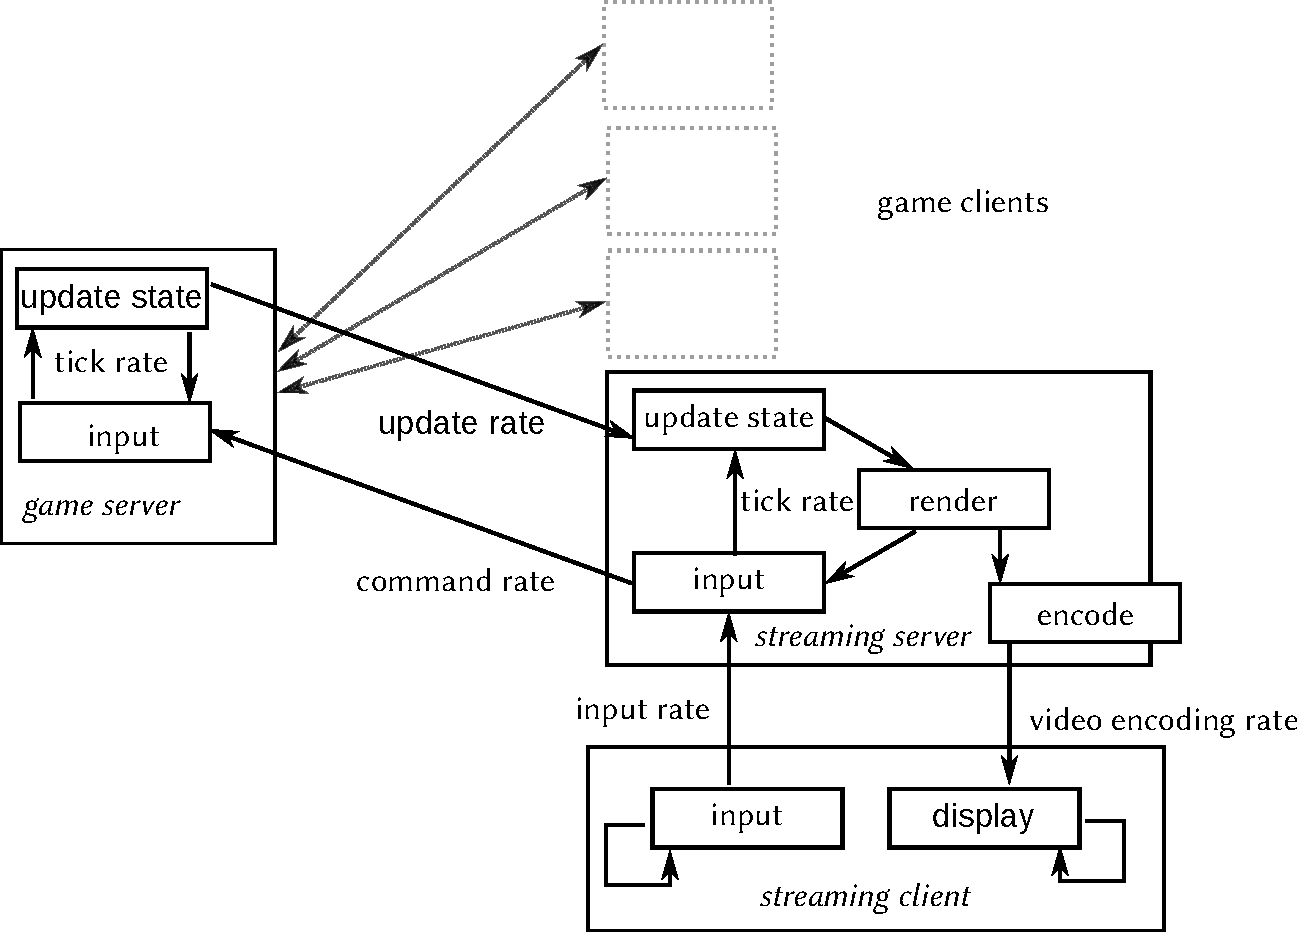
\includegraphics[width=1.0\columnwidth]{images/game-tick-rate-streamed.pdf}
	\caption{Interaction of client and server in streamed online games.}
\label{fig:tickrate-streamed}
\end{figure}


%%%%%%%%%%%%%%%%%%%%%%%%%%%%%%%%%%%%%%%%%%%%%%%%%%%%%%%%%%%%%%%%%%%%%%%%%%%%%%%%
\subsection{Sources of Latency in Gaming}
\label{sec:latency}

It is evident that latency is a critically important factor for online 
games, for fast games, or especially for competitive games as will be 
discussed in Sec.~\ref{sec:game-criteria}. But besides the obvious 
network delay there are many more sources of delay that need to be 
factored in when examining these games, including the input device, the 
time to sample and process the input, the game engine and server and 
their tickrates, frame rendering time, and ultimately the time to 
display the frame on the monitor. Only if all sources are factored in 
the complete \textbf{end-to-end lag} is captured. What makes matters 
even worse, is that this lag is usually not constant but can vary 
depending on the type of action triggered by the input. While some 
simple actions, say opening the menu, may have a very short lag, more 
complex interactions, e.g., issuing a move command, may take 
considerable longer to complete especially when the game is not 
performing well, partly due to the actions taking more than one game 
tick to complete. Therefore, each video game will have a distinct ``lag 
profile''.  Fig.~\ref{fig:tickrate-timeseries} shows a time series 
attempting to exemplify this for the simplified case of an online video 
game.


\begin{figure}[!t]
	\centering
	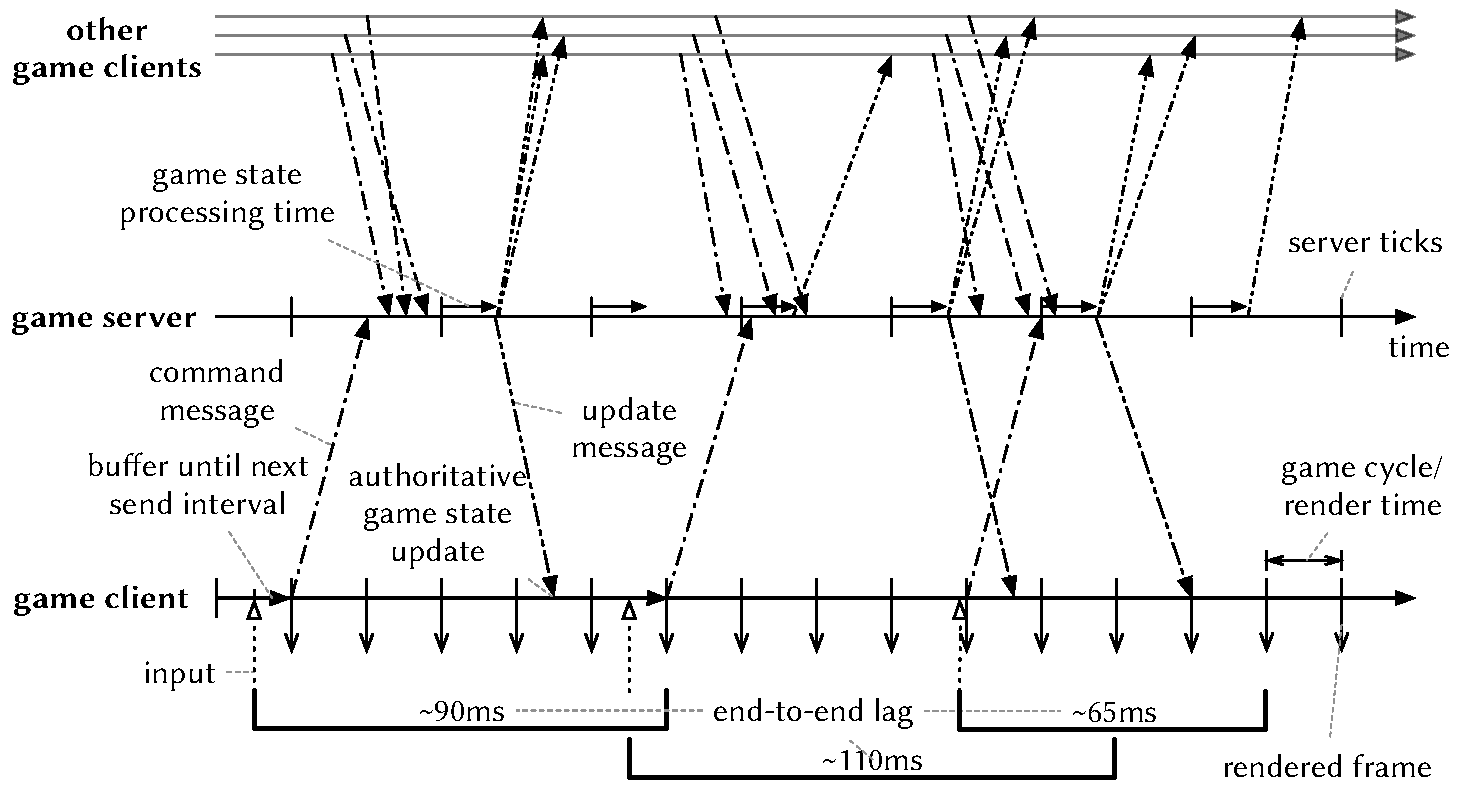
\includegraphics[width=1.0\columnwidth]{images/tickrate-timeseries.pdf}
	\caption{Exemplary time series of an online video game's client-server 
interaction and resulting end-to-end lag. Delay values are given for a 
framerate of \SI{60}{\hertz} and a server tickrate of \SI{30}{\hertz}, 
the network latency will only show minor variations.}
\label{fig:tickrate-timeseries}
\end{figure}

To demonstrate the effects of all the involved parameters, a 
MATLAB-based queuing simulation closely resembling the interactions 
given in Fig.~\ref{fig:tickrate-timeseries} was set up. With this the 
influence of any of the lag sources can be easily simulated and the 
biggest culprits identified. For example, the influence of the 
framerate on online games becomes evident in 
Fig.~\ref{fig:e2e-delay-sim}, where increasing the framerate from 
\SI{15}{\hertz} up to \SI{120}{\hertz} can significantly reduce the 
game's lag, a result that can also be easily applied to cloud games, 
where streaming often operates at a lower framerate to conserve 
bandwidth.

%All in all, if possible, video game measurements should always 
%consider the full \textbf{end-to-end} lag factoring in every possible 
%source of delay but also the presence latency compensation and 
%concealment techniques.


\begin{figure}[!t]
	\centering
	%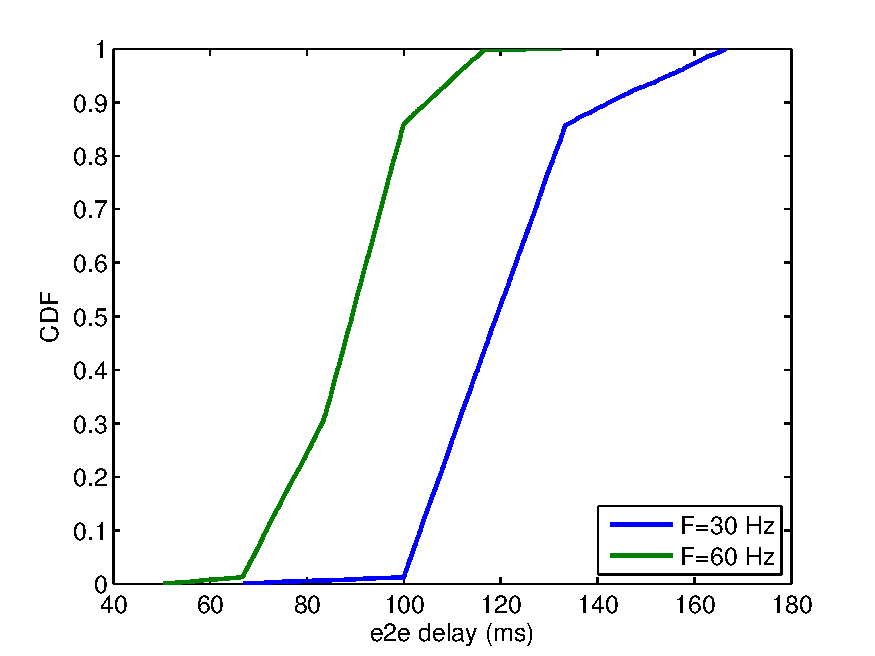
\includegraphics[width=1.0\columnwidth]{images/e2e-delay-sim.pdf}
	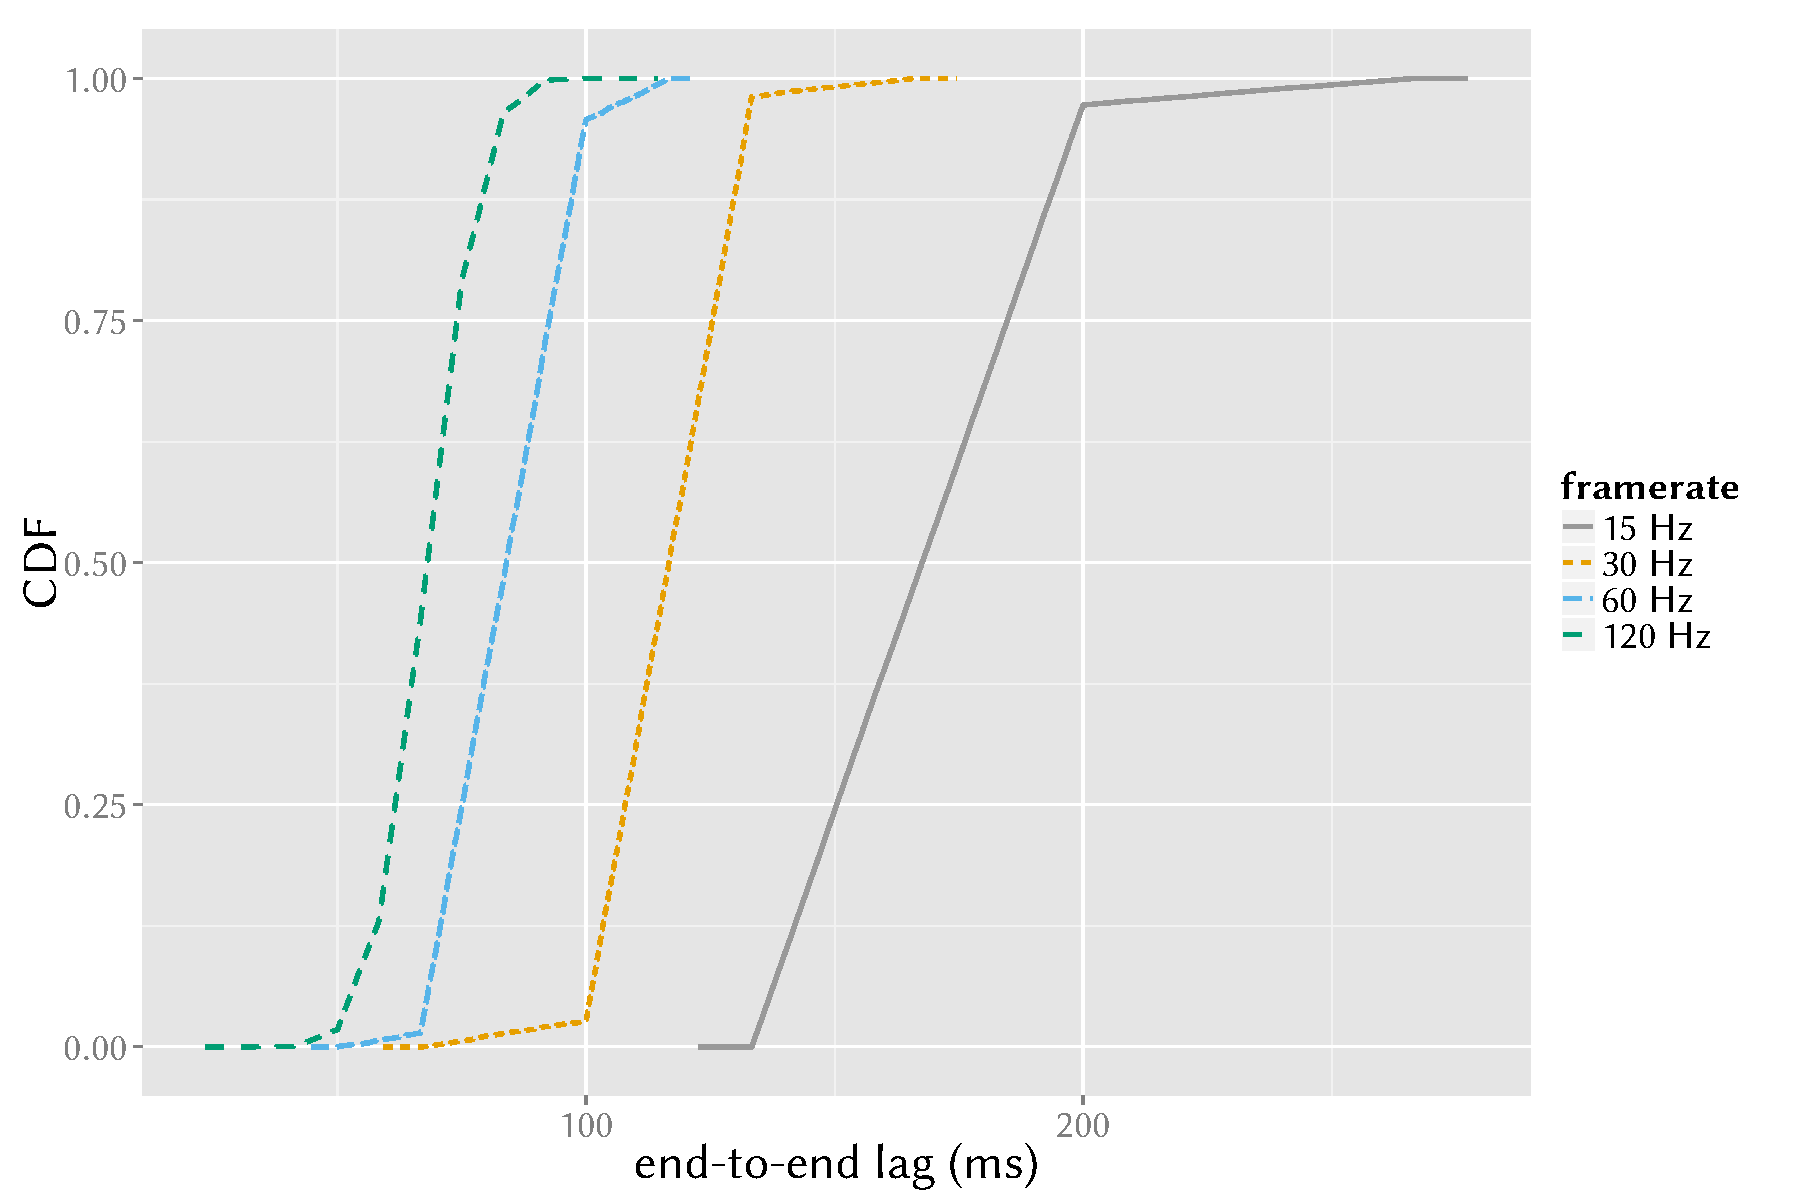
\includegraphics[width=1.0\columnwidth]{images/R-gamesim.pdf}
	\caption{\acrshort{ECDF} of a simulated online video game interaction 
and the resulting end-to-end lag depending on the game's frame rate. 
One-way network delay followed a Gaussian distribution with $\mu = 
\SI{20}{\milli\second}$ and $\sigma = \SI{5}{\milli\second}$. The 
server's tickrate was set to \SI{60}{\hertz}.}
\label{fig:e2e-delay-sim}
\end{figure}




% Online games attempt to compensate network latency through various 
%means, such as already showing the results of your local inputs while 
%waiting for the authoritative update from the server and potentially 
%rolling back the local updates.

% TODO: Also mention lag compensation/concealment techniques:
% Client-side: non-authoritatively update game state based on own 
%inputs and merging it afterwards with the server's view, correcting any 
%prediction errors
% Server-side: Keep a short history of past game states, and do not 
%execute player commands at the state they were received but rather at 
%the (estimated) state time they were intended for.

% lag compensation can also be implemtented specifically for cloud 
%gaming as the work conducted in \cite{Lee:2015:OUS:2742647.2742656} 
%suggests, however incurring siginficant overhead in terms of processing 
%time for the game logic and renderer as well as the encoding and 
%bandwidth due to specutatively generating and transmitting frames ahead 
%of their corresponding input.


% game keeps history of recent game state snapshots to interpolate 
%between two server states and create a smoother experience (thus 
%decoupling client frame rate from the server's state updates), but adds 
%e.g. \SI{100}{\milli\second} of view lag due to snapshot history.


%%
%\subsubsection{Online Video Game Latency Concealment Techniques}


% input: absolute (eg mouse) vs. relative (analog stick)
% frame perfect input
% double/triple buffering
% inputs per minute vs timing precision of input
% range of interactivity
% latency sensitivity/responsiveness of different game mechanics / UI 
%elements in the same game
% latency of camera movement / UI vs actual game elements


%Info on source engine networking: 
%\url{https://developer.valvesoftware.com/wiki/Source_Multiplayer_Networking}
%\url{https://developer.valvesoftware.com/wiki/Latency_Compensating_Methods_in_Client/Server_In-game_Protocol_Design_and_Optimization}
%(Latency Compensating Methods in Client/Server In-game Protocol Design 
%and Optimization, Yahn W. Bernier (yahn@valvesoftware.com), 2001, 
%Software Development Engineer, Valve Software)



% Online games generally follow one of two designs. Either there is a 
%dedicated server available to host the game, or one of the clients is 
%elected to additionally act as the server.
% The election is typically based on criteria such as the available 
%performance and latency. If the selected host drops out of the game, a 
%new server has to be elected and the game gets migrated there, usually 
%stopping the game for a few moments. Competitive games almost always 
%choose the dedicated approach to ensure fairness, stability and better 
%control cheats.



% \begin{figure*}[!t]
% 	\centering
% 	\begin{subfigure}[b]{0.5\textwidth}
% 		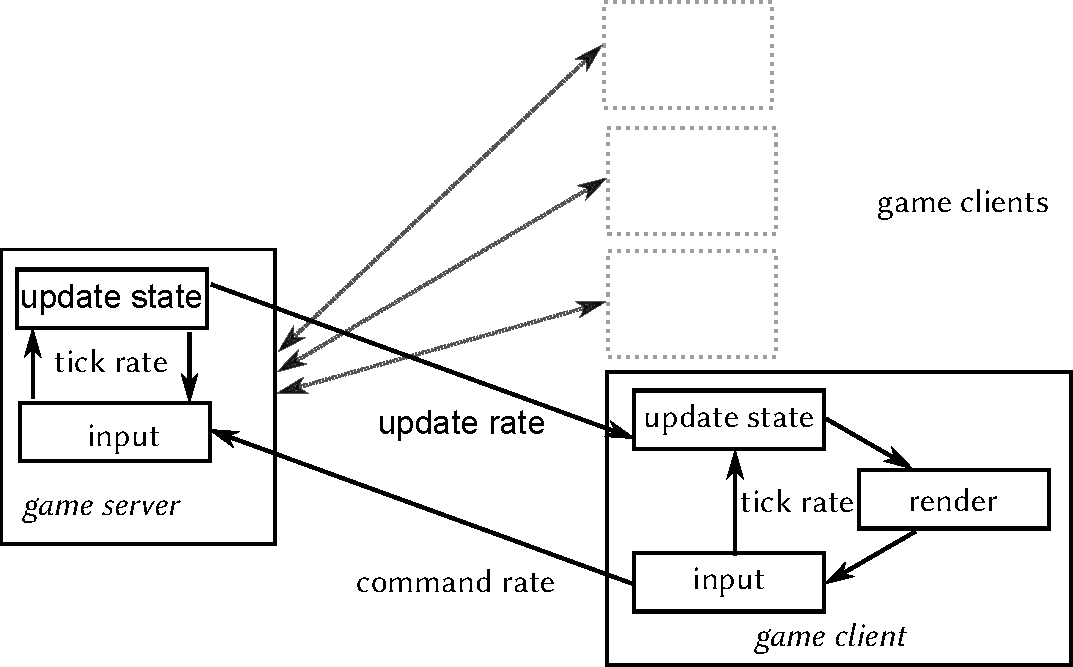
\includegraphics[width=1.0\columnwidth]{images/game-tick-rate.pdf}
% 		\caption{In typical online games.}
% 		\label{fig:tickrate-online}
% 	\end{subfigure}%
% 	~
% 	\begin{subfigure}[b]{0.5\textwidth}
% 
%		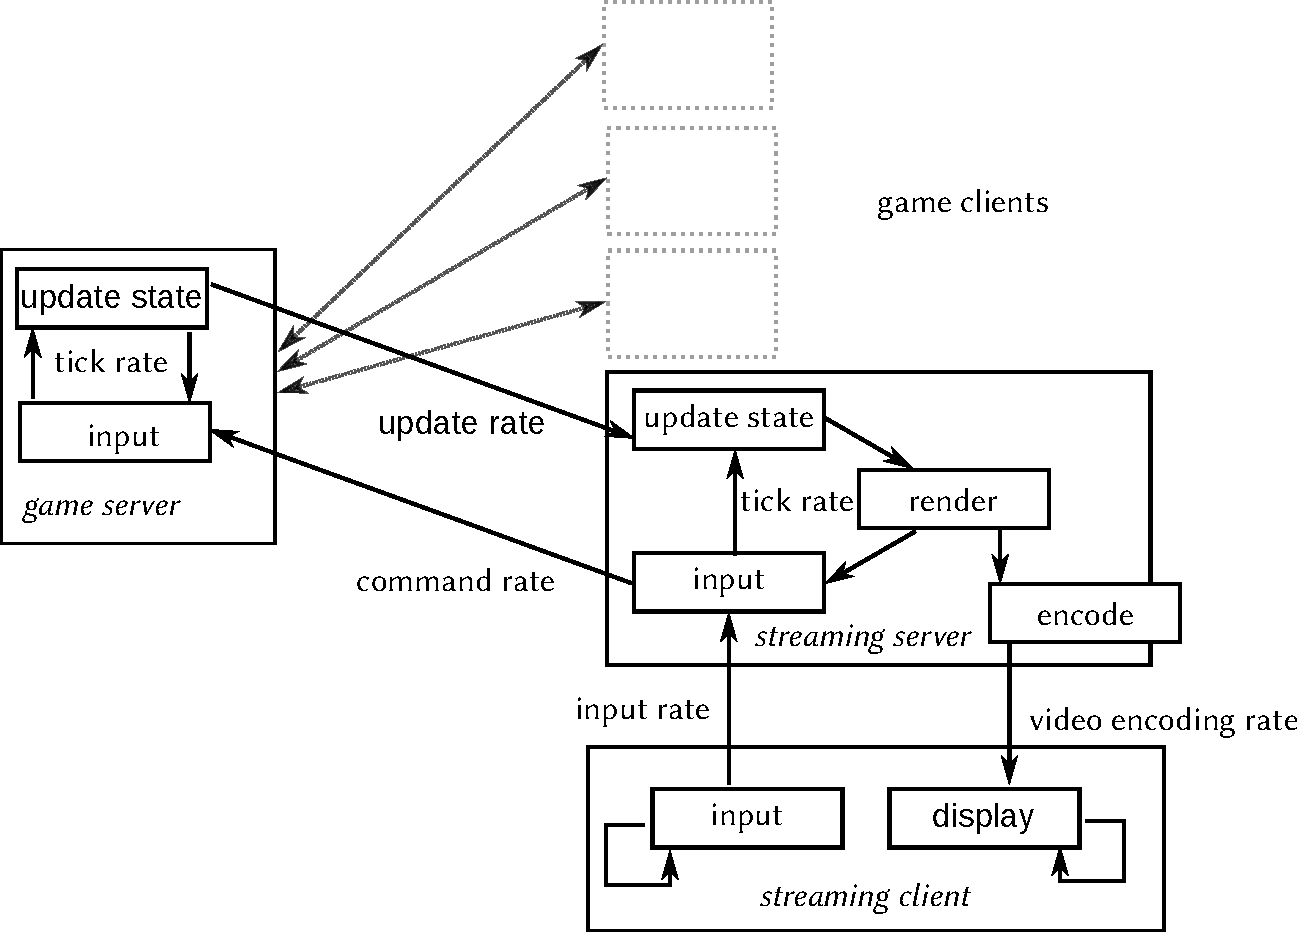
\includegraphics[width=1.0\columnwidth]{images/game-tick-rate-streamed.pdf}
% 		\caption{In a cloud gaming scenario.}
% 		\label{fig:tickrate-streamed}
% 	\end{subfigure}
% 	\caption{Interaction of the game client and server.}
% 	\label{fig:tickrates}
% \end{figure*}



% \begin{figure}[!t]
% 	\centering
% 	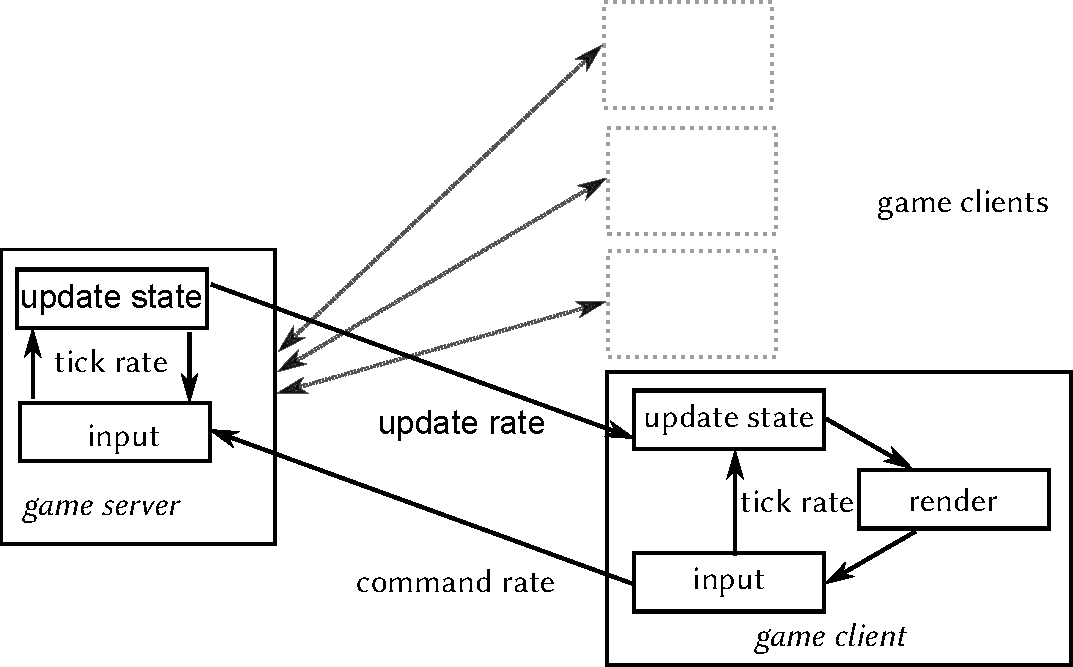
\includegraphics[width=1.0\columnwidth]{images/game-tick-rate.pdf}
% 	\caption{Interaction of client and server in typical online games.}
% \label{fig:tickrate-online}
% \end{figure}





% \begin{table}[!t]
% \caption{Exemplary table of some competitive and popular video game 
%tickrates that are either known, speculated upon, or derived by 
%counting update and command messages. Much of this information here is 
%guesswork from sometimes dubious sources and needs to be verified.}
% \label{tbl:tickrates}
% 	\centering
% 	\begin{tabu}{X[0.45]|X}
% 		\toprule
% 		\textbf{Video Game} & \textbf{Tickrate} \\
% 		\midrule
% 		CS: GO & Configurable \SI{64}{\hertz}/\SI{128}{\hertz} \\ \midrule
% 		Battlefield 4 & \SI{30}{\hertz} (\SI{10}{\hertz} for state outside 
%of close proximity to player). \SI{60}{\hertz}/\SI{120}{\hertz} 
%implemented on test servers. \\ \midrule
% 		Minecraft & max. \SI{20}{\hertz} \\ \midrule
% 		League of Legends & \SI{30}{\hertz} (guessed) \\ \midrule
% 		Dota 2 & \SI{30}{\hertz} \\ \midrule
% 		StarCraft II & supposedly either \SI{16}{\hertz} or \SI{32}{\hertz} 
%\\ \midrule
% 		Eve Online & \SI{1}{\hertz} \\ \midrule
% %		Sports Game 1 & \\ \midrule
% 		Project Cars & \SI{600}{\hertz} (Physics) \SI{250}{\hertz} (Input) 
%\\ %https://twitter.com/projectcarsgame/status/551340759858040833
% 		\bottomrule
% 	\end{tabu}
% \end{table}



% \subsection{Determining Video Game Popularity and Engagement}
% FUTURE WORK!

% Using Steam data as a popularity measure and get a grasp of which 
%games could be worthwhile to look at. Ties in to user engagement 
%metrics to determine the quality a game delivers in a current 
%situation. Alternative view: the more engaged players are to a game, 
%the more important is delivering a good quality (e.g. for streaming).

% For example, there might be a correlation between a game's price and 
%the average time it's been played, as 
%Figure~\ref{fig:tickrate-streamed}.


% Other  k-means clustering of steam/price data or other graphs

% \begin{figure}[!t]
% 	\centering
% 
%	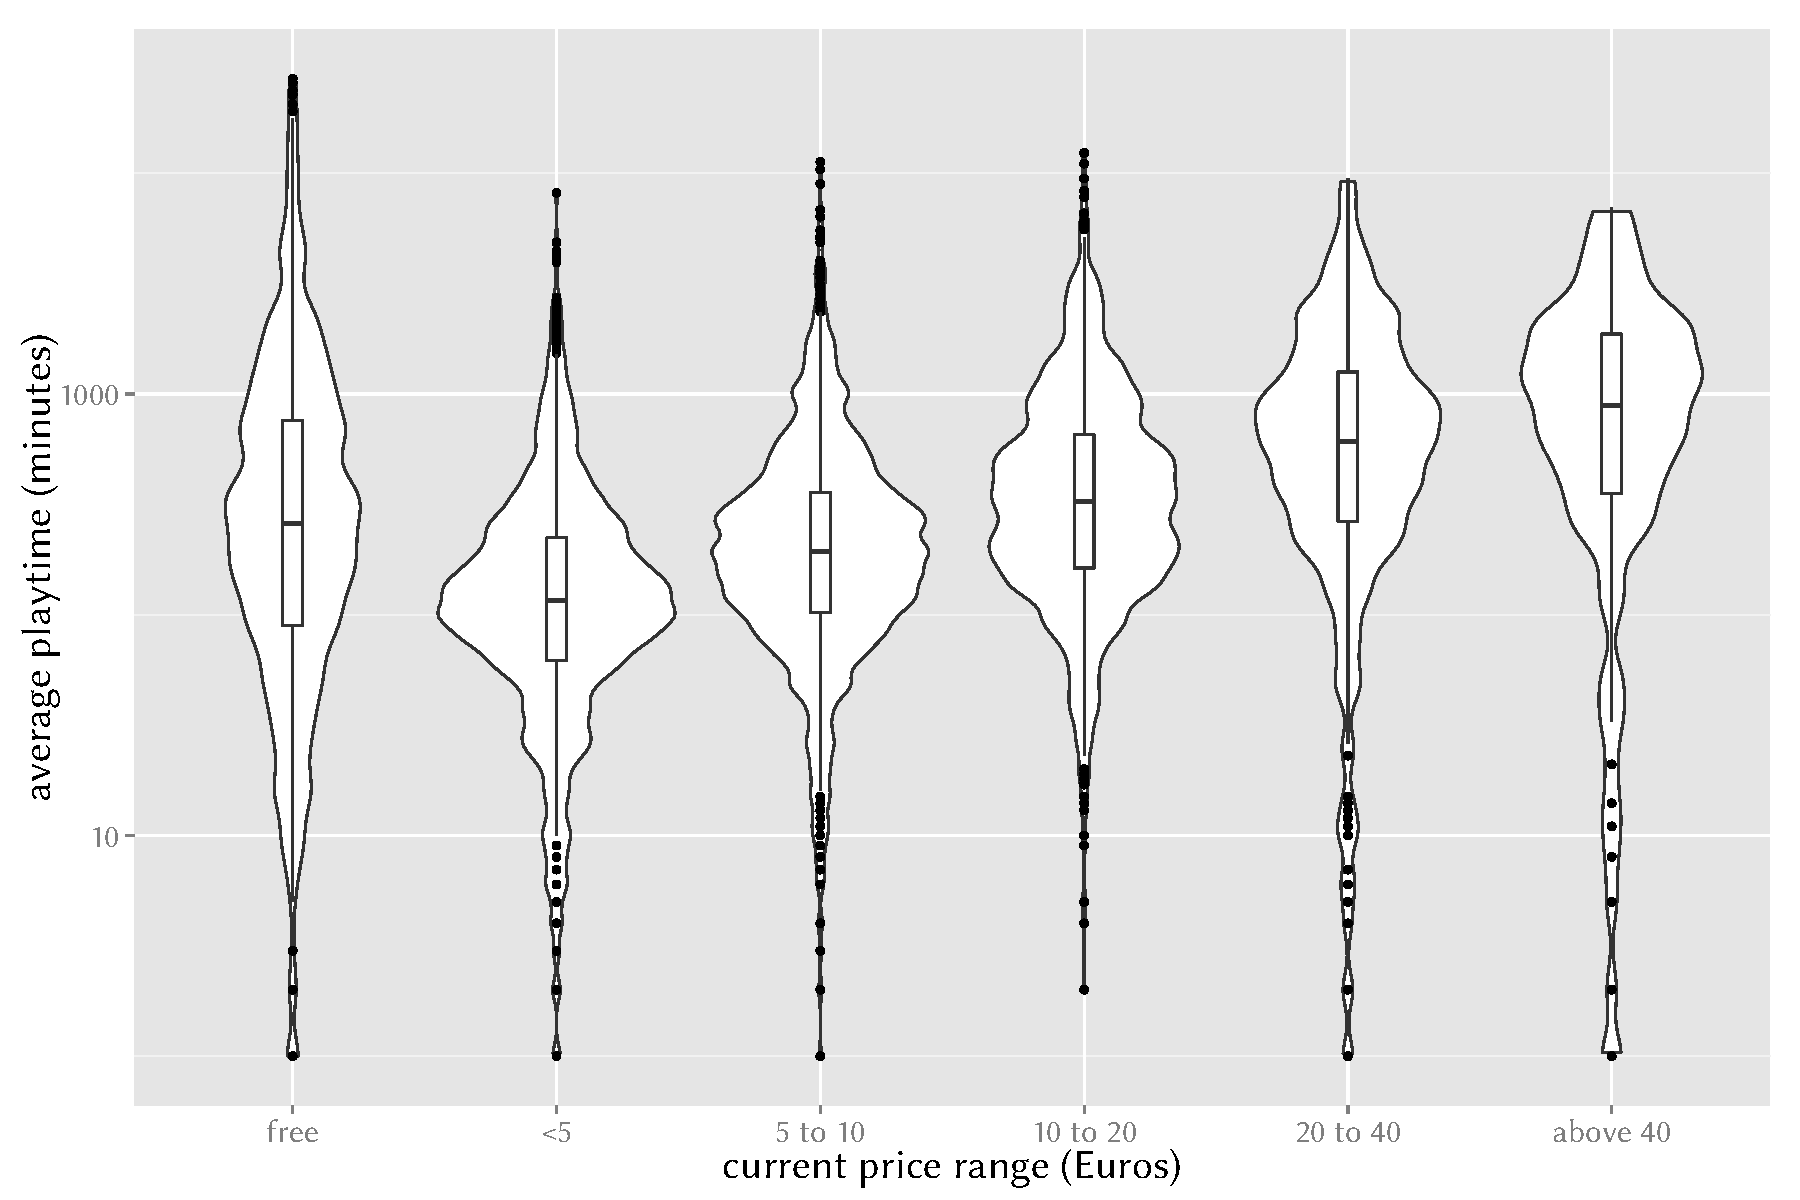
\includegraphics[width=1.0\columnwidth]{images/dampfviolinen-playtime.pdf}
% 	\caption{Game cost as a possible categorization and engagement 
%factor. Displayed is a violin plot of the current costs in relation to 
%the average playtime of individual games.s}
% \label{fig:cost-playtime-violin}
% \end{figure}

% Categorization dimensions viable for measuring online video game 
%quality:



%\footnote{\url{http://accidentalscientist.com/2014/12/why-movies-look-weird-at-48fps-and-games-are-better-at-60fps-and-the-uncanny-valley.html}}
%\url{https://stackoverflow.com/questions/17411/how-do-you-separate-game-logic-from-display}
%\url{http://higherorderfun.com/blog/2010/08/17/understanding-the-game-main-loop/}

%!TEX root = paper.tex
%%%%%%%%%%%%%%%%%%%%%%%%%%%%%%%%%%%%%%%%%%%%%%%%%%%%%%%%%%%%%%%%%%%%%%%%%%%%%%%%
\section{Conducting Measurements}
\label{sec:measurementgoals}

Before proposing actual measurement methods, three equally important aspects relating to any game measurement approch are discussed: the metrics to evaluate, the parameters to use, as well as the selection of games. 

Finding fitting objective \gls{QoE} metrics is strongly game-dependent. They need to reflect the game's mechanics in a meaningful manner. But this is beyond the scope of this paper, which will only concern itself with game-independent metrics, of which three are considered here: The framerate, the frame \gls{IAT}, and the end-to-end lag (or parts thereof as some measurement methods might not be able to record the full lag).

The framerate and \gls{IAT} are a good representation for the game's fluidity and responsiveness to inputs and are especially important to note for cloud gaming. The end-to-end lag gives the best overall picture on the attainable gaming experience and should always be preferred over partial lag values, such as purely investigating the network latency. The impact of the lag also depends on the type and precision of controls the game offers. A keyboard and mouse driven PC game might be much more sensitive to high lag than a mobile game with touch controls.

Input controls are but one aspect of the games environment and settings, which also need to be carefully selected to achieve meaningful results. This especially concerns PC games which usually offer a wide range of options to choose from of which the graphics options are the most impactful. The recommended settings to run games at are a video resolution of 1080p or higher with the games other graphics options set to high or at lest medium values in order to reflect a typical gaming experience. The test computers should be able to deliver these graphical settings at a framerate of \SI{60}{\hertz} which is considered the minimum rate for many players. Some types of games are less dependent on the framerate, where a rate of \SI{30}{\hertz} is considered acceptable. Experimenters should never set a framerate lower than that for the reasons discussed in the previous section. They should however also consider testing at higher framerates, especially for competitive games with a high tickrate to further reduce the negative impact of low framerates.


%%%%%%%%%%%%%%%%%%%%%%%%%%%%%%%%%%%%%%%%%%%%%%%%%%%%%%%%%%%%%%%%%%%%%%%%%%%%%%%%
\subsection{Choosing Representative Games}
\label{sec:game-criteria}

%The general focus here lies on measuring online games with high demands. The idea is that if these games work at an objectively good quality, it is reasonable to assume that all other games do so as well. 
It is quite difficult to find games that are representative for certain input and lag demands. For example, the traditional game genre categorization is not a good starting point as games from the same category can be vastly different in terms of game speed and necessary reaction times. Rather, the following four metrics might be more helpful to assess a game's applicability for measurements.

 \begin{itemize}
    \item \textbf{Required number of decisions or actions in a certain time span.} E.g., the \gls{CCG} \textsc{Hearthstone} may only require a handful of actions (i.e., choosing and playing cards) each turn, while in order to competitively play the \gls{RTS} \textsc{Starcraft 2} you more or less need to achieve a few hundred so-called \gls{APM}, with the record being higher than $800$ \gls{APM}.% \cite{6404025} defines a related metric dubbed \textit{command heaviness} comparing the amount of change to the input rate, under the umbrella term \textit{real-time strictness}. This ties in with the concepts of game sense. Micromanagement-intense games usually tend to result in high APM rates.

    \item \textbf{Maximum successful reaction time to in-game actions.} Again e.g., \textsc{Hearthstone} as a turn-based game requires no instant reaction time at all, as the opponent's and the player's actions are separated into turns. First-person shooters like \textsc{Counter-Strike: Global Offensive} are usually on the opposite extreme of this spectrum, as they tend to have a very high tickrate and literally often require you to ``shoot first'' to win. This is also investigated/defined in \cite{Claypool:2006:LPA:1167838.1167860}. This metric is also closely related to the next item.

    \item \textbf{(Un-)Predictability of actions.} Compare, e.g., an entirely rhythm-based game (e.g., \textsc{Guitar Hero}), where you can completely pre-plan all of your actions, to a twitch-based shooter like \textsc{Counter-Strike} where you have to react from moment to moment. In theory, a game with no surprising events will be much less influenced by a higher end-to-end lag.

    \item \textbf{Accuracy and precision of input actions.} Accuracy can be both in terms of temporal as well as spatial aspects which can be influenced by both the image quality and the frame rate.  %Commands through keybindings usually require less precision than freeform mouse inputs on certain regions on the screen.

\end{itemize}


%%%%%%%%%%%%%%%%%%%%%%%%%%%%%%%%%%%%%%%%%%%%%%%%%%%%%%%%%%%%%%%%%%%%%%%%%%%%%%%%
%%%%%%%%%%%%%%%%%%%%%%%%%%%%%%%%%%%%%%%%%%%%%%%%%%%%%%%%%%%%%%%%%%%%%%%%%%%%%%%%
\subsection{Measurement Approaches}
\label{sec:measurementapproaches}

With these metrics, test parameters, and categorizations in mind, one can now attempt to conduct the actual measurements of which there are three distinct methods each situated at a unique vantage point as depicted in Fig.~\ref{fig:measurement-methods}.

\begin{figure}[!t]
    \centering
    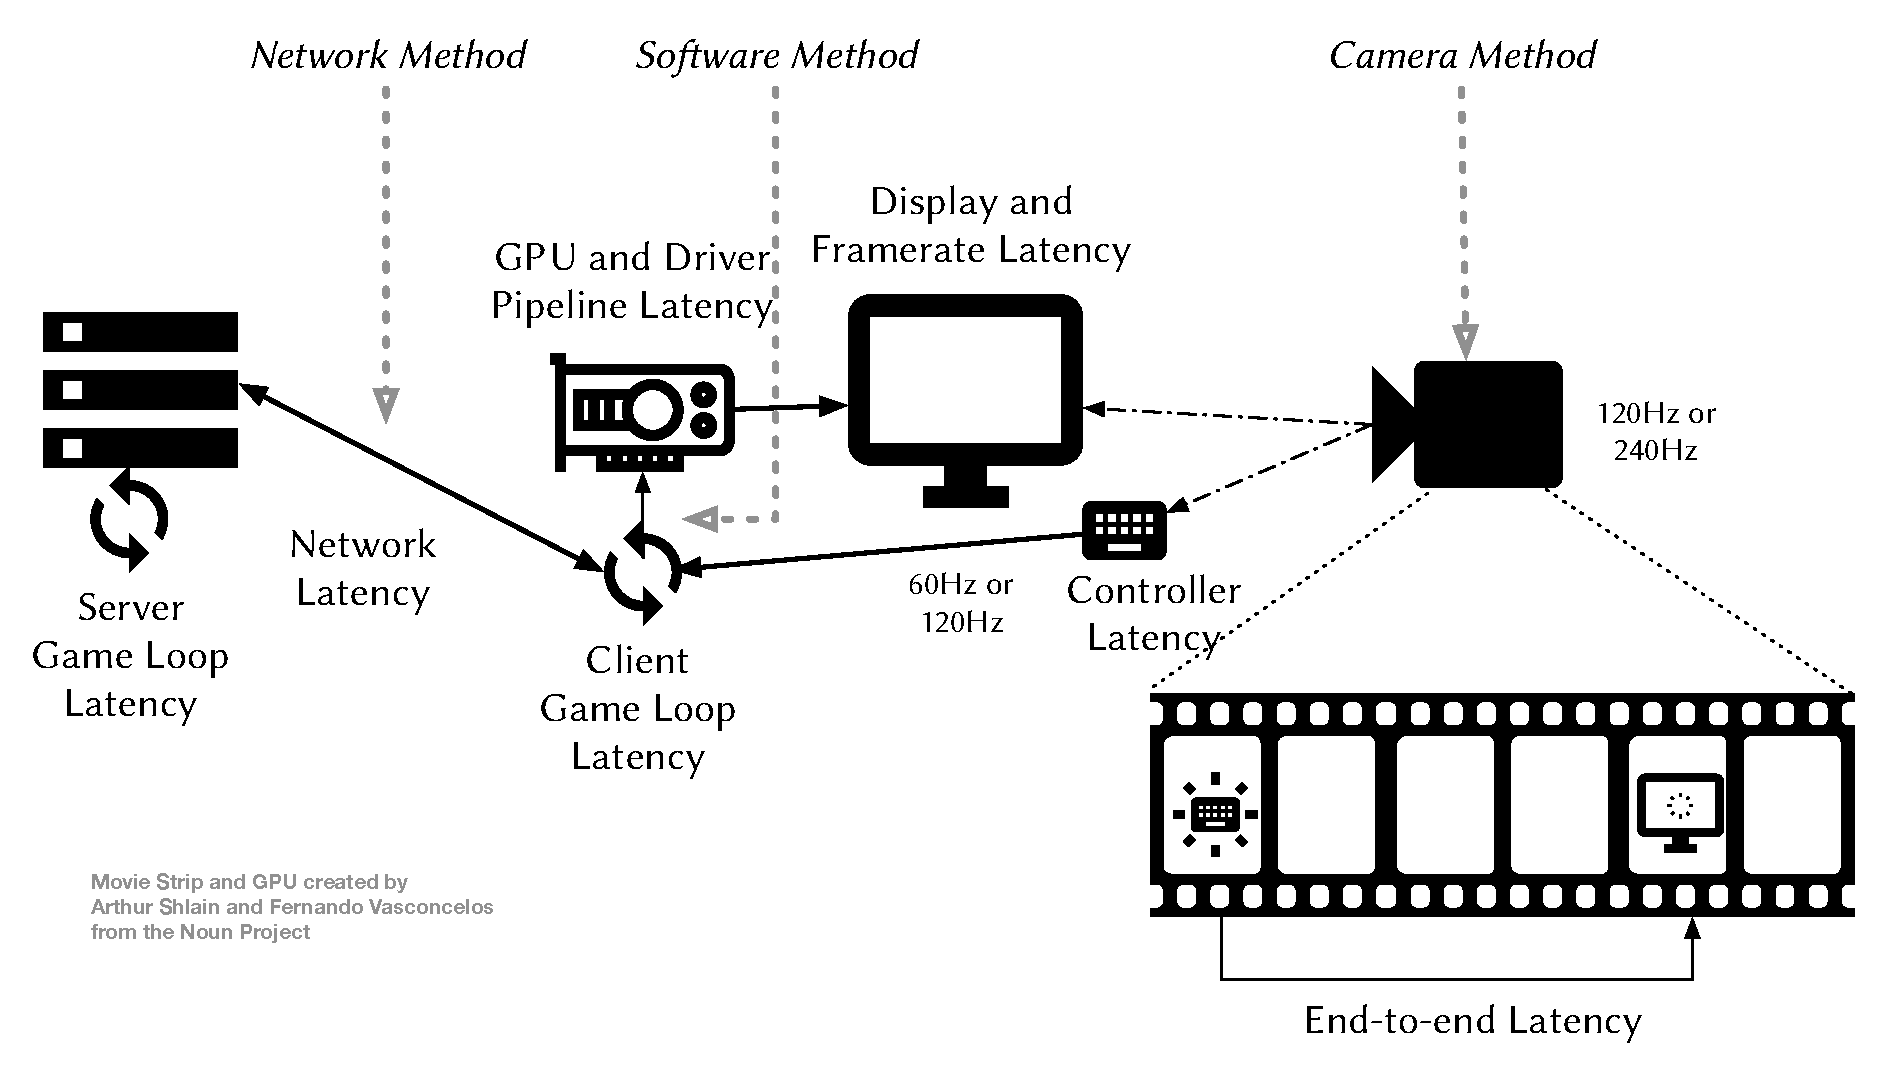
\includegraphics[width=1.0\columnwidth]{images/e2e-lag.pdf}
    \caption{Location of the three measurement approaches to capture end-to-end latency inside a usual online video game lag chain.}
\label{fig:measurement-methods}
\end{figure}


%%%%%%%%%%%%%%%%%%%%%%%%%%%%%%%%%%%%%%%%%%%%%%%%%%%%%%%%%%%%%%%%%%%%%%%%%%%%%%%%
\subsubsection{Screen Recording Software Method}

Recording the output stream of a video game might be the simplest approach. It can capture both the framerate and \gls{IAT} at a driver level, and the recorded video can be used for image and quality analyses as well as to correlate it to additionally recorded input events to calculate the lag. This is not the the complete end-to-end lag however, as both the controller and screen output latency are missing. The need to install additional software might make it unsuitable for some scenarios, e.g., when measuring console video games. As a variant of this method, one can also record the output stream with a video capture card on a secondary computer, which does not negatively effect the game's performance as the software method does.

Examples of this approach include both \cite{Chen:2011:MLC:2072298.2071991} and \cite{6670099} which measured the end-to-end latency of cloud gaming services in the game client. They do this by invoking the system menu in games and measuring the time until it is displayed. A 2013 paper \cite{6574660} investigates the quality of cloud gaming interactiveness (i.e., the lag) as well as image quality by employing software recording methods on the client's computer.
%However, this method assumes a constant delay of game actions and may not capture the actual end-to-end lag of many of real game actions, as they are typically different from and longer as the latency of displaying a menu. A 2013 paper \cite{6574660} investigates the quality of cloud gaming interactiveness (latency) as well as image quality by employing software recording methods on the client's computer. With these techniques the challenges regarding the quality are discussed.


%%%%%%%%%%%%%%%%%%%%%%%%%%%%%%%%%%%%%%%%%%%%%%%%%%%%%%%%%%%%%%%%%%%%%%%%%%%%%%%%
\subsubsection{Passive Network Measurements}

In some cases it may also be advantageous to tap into the network interactions of the games and record the command and update messages sent between server and clients. While this is not a direct measure of game quality, it can give insights into the game's inner workings, such as the tick rates, and one can derive, e.g., the lowest achievable end-to-end lag from this.

%Can only investigate command and update messages, not tick rate directly. Evaluate rate, IAT, and bandwidth, estimate latency (though there may be no direct link between commands and updates).

Besides simple flow-based or packet-counting network metrics, many games also allow for deeper packet-dissecting analyses, as the often rely on standardized protocols or data formats, such as Protobuf\footnote{\url{https://developers.google.com/protocol-buffers/}} or incorporate well-known third-party multiplayer-enabling libraries. %And cloud games sometimes use derivates from the RTP-family or XMPP-based(VERIFY) protocols. 
Additionally, almost no game encrypts its time-critical messages, enabling an easy read-out. Through these means, the specific commands can be read from the network and potentially linked to their effect on the game state in the corresponding state update messages.
%, but also potentially allowing malicious actions to be taken easily.


%%%%%%%%%%%%%%%%%%%%%%%%%%%%%%%%%%%%%%%%%%%%%%%%%%%%%%%%%%%%%%%%%%%%%%%%%%%%%%%%
\subsubsection{Camera Recordings}

The only method to fully capture the end-to-end lag is to simultaneously record both the screen and input device through an external camera. The experimenter then has to count the frames between pressing a button on the input device and the action appearing on the screen and calculate the lag from this. For better visibility the input device is usually modified with an LED that turns on when the button is pressed. Also, the camera should operate at least at twice the monitor's refresh rate according to the Nyquist-Shannon sampling theorem. An additional benefit of this method is, that the game and the computers remain unaltered and are therefore not affecting any game mechanics. This approach is often used in the gaming press and by game developers to evaluate a game's control fidelity. A variant of this approach, replacing the camera with a photodiode and synthetically creating the input events with a microcontroller is described in \cite{beyermethod}, though it may be difficult to use for certain game actions that have a barely visible or unpredictable on-screen effect.


% Ultimately, to capture any and all latency sources in gaming you would need to rely on external recording gear.
% With modified input: zero latency and visible input detection (e.g. solder some LEDs to the buttons)

% Also Arduino with photodiode method described in \cite{beyermethod}
% Both this and camera method also work for closed game consoles


%%%%%%%%%%%%%%%%%%%%%%%%%%%%%%%%%%%%%%%%%%%%%%%%%%%%%%%%%%%%%%%%%%%%%%%%%%%%%%%%
%\subsection{Evaluated Metrics}

%%%%
%\subsubsection{Frame Rates and Frame Times (i.e. frame IAT)}
%i.e. frame IAT
%Reasoning for frame IAT and the negligence of past investigations
%%%%
%\subsubsection{Total and additional end-to-end latency}
%physical controller input to in-game reaction
%different in-game actions have already difference in latency, therefore need to test various actions for a complete picture
%Also discuss RTT as Hz (1/RTT) as measure for interactivity


%%%%%%%%%%%%%%%%%%%%%%%%%%%%%%%%%%%%%%%%%%%%%%%%%%%%%%%%%%%%%%%%%%%%%%%%%%%%%%%%
%\subsection{Reasonable Configuration/Setting Ranges to Test}

% Resolution: Minimum 720p, 1080p recommended, even higher is better (1440p or 2160p)
% Frame rate: 60 fps very much recommended, 30 absolute minimum,  120 or 144 can also be feasible
% Configure games to run at high or at least medium settings
% For console games: use the games intended settings for the console, never downscale the game or reduce the frame rate for streaming
% Assume no network latency higher than 200ms, preferably less than 100ms
% Assume typical access link conditions, i.e. no less than 10-16Mb/s



%Works only for general purpose computing devices with full access.
%Easiest method, but might not capture full end-to-end latency.
%FRAPS, OBS, DirectX Hooking, MSI Afterburner
%FCAT as hybrid solution with external capture card and computer


% \url{http://www.red.com/learn/red-101/high-frame-rate-video}


% articles:
% why frametimes
%     \url{https://techreport.com/review/21516/inside-the-second-a-new-look-at-game-benchmarking}

% Inside the second with Nvidia's frame capture tools
%     \url{https://techreport.com/review/24553/inside-the-second-with-nvidia-frame-capture-tools}

 % As the second turns: the web digests our game testing methods
 %    \url{https://techreport.com/blog/24133/as-the-second-turns-the-web-digests-our-game-testing-methods}

% GPU Reviews: Why Frame Time Analysis is important
%     \url{http://www.vortez.net/articles_pages/frame_time_analysis.html}

% Durante's Witcher 3 analysis: the alchemy of smoothness
%     \url{http://www.pcgamer.com//durantes-witcher-3-analysis-the-alchemy-of-smoothness/}


% Analysing Stutter – Mining More from Percentiles
%     \url{https://developer.nvidia.com/content/analysing-stutter-%E2%80%93-mining-more-percentiles-0}

% fraps vs fcat method
%     \url{http://www.extremetech.com/gaming/154089-after-almost-20-years-gpu-benchmarking-is-moving-past-frames-per-second}

% FRAPS + FRAFS
% \url{http://www.fraps.com/}
% \url{http://sourceforge.net/projects/frafsbenchview/}
% \url{http://www.5group.com/wordpress/2012/07/14/gpu-mist-pre-release-1-0-rc1/}

% issue: Fraps measures the flip queue input rather then the actual render output frames which is fine when measuring FPS but is rather poor if you want to measures actual frame times and analyze microstutter.


% NVIDIA FCAT
% \url{http://www.geforce.com/hardware/technology/fcat}
% \url{http://www.overclockers.com/nvidias-fcat-gpu-testing-pursuing/}


% Valve for Linux GL Games
% \url{https://github.com/ValveSoftware/voglperf}

% Info über MSI Afterburner overlay? oder GF experience? GPU-Z? Rivatuner Statistics Server?
% \url{http://www.overclock.net/a/how-to-use-rivatuner-afterburner-on-screen-display-and-more}



% \url{https://en.wikipedia.org/wiki/Game_classification}
% \url{https://en.wikipedia.org/wiki/Video_game_genre}
% \url{https://en.wikipedia.org/wiki/List_of_video_game_genres}


%!TEX root = paper.tex
%%%%%%%%%%%%%%%%%%%%%%%%%%%%%%%%%%%%%%%%%%%%%%%%%%%%%%%%%%%%%%%%%%%%%%%%%%%%%%%%
\section{Conclusion}
\label{sec:conclusion}

%These scenarios reveal the necessity of a tight control over game parameters, such as the framerate, resolution, or input devices, in accordance with the game's type.

This paper presents a model for \acrfull{E2E} lag in video games, including online and cloud variants. The \gls{E2E} lag represents the time elapsed between a player input event such as mouse movement or keystrokes and the display of the event's results in the game on the local display. This lag is a main governing factor for \acrfull{QoE} in human-computer interaction in general, and video games in particular. The model is parameterized on the command rate at which batched user events are processed, the server tickrate and state processing time, the game's local framerate, the network delay (for online games), and codec delays (for cloud games). % Note: We don't look at local latencies really: Mice and keyboards, USB, TV sets, multibuffering, ...
The model is simulated using \acrfull{DES}, showing the dominant influence of the game framerate on the \gls{E2E} lag particularly for low framerates. This contribution to \gls{E2E} lag may even mask the influence of network delay, yet it appears underrepresented in previous work.  On an abstracted level, the model helps to explain the mechanics behind lag in different game types and architectures. This is of interest to both actual implementations of games and study design for game \gls{QoE} assessment. To foster participation, the model simulation code used for this paper is available as free, open-source software from the authors' repository~\cite{onlinegame-lag-sim-repo}, as are the raw data.
%
%results, meta: explains lag mechanics, helps judge correctness of qoe models
%results, numbers: parameter study for local, online, cloud games.
%
%fuwo: use this to make better studies
%
%
%, , is an important influence 
%The \acrfull{QoE} of depends partially on the lag 
%The models presented here serve to provide initial insights into the complex interactions of \gls{E2E} game lag. Although the underlying abstract model adopts some simplifications and some properties are not incorporated yet, the results are still very revealing. Using the model and simulator as baseline, one can get a good estimation of the expected video game \gls{QoS} values. 
%%Alternatively, it can help in choosing representative games for select scenarios.
%A proper setup of gaming \gls{QoS}/\gls{QoE} studies is of critical importance to their validity. The \gls{E2E} lag queuing model set up in this work can support these endeavors a long way through an improved understanding of relevant game properties and their interactions. The role of the framerate, and its lag-inducing effects has been undervalued in the past, which these models and simulations aim to rectify. Of special interest is the masking effect low values of the framerate or tickrate have on the network delay on the \gls{E2E} lag. This and similar side effect need to be considered for subsequent research efforts.

\printbibliography 

\end{document}
